\documentclass[a4paper]{article}
\usepackage[spanish]{babel}
\usepackage[utf8x]{inputenc}
\usepackage{fancyhdr}
\usepackage{charter} % tipografia
%\usepackage{graphicx}
\usepackage[pdftex]{graphicx}
\usepackage{bm} % bold font in math mode
\usepackage{sidecap}
\usepackage{adjustbox}
\usepackage{caption}
\usepackage{subcaption}
\usepackage{booktabs}
\usepackage{makeidx}
\usepackage{float}
\usepackage{amsmath, amsthm, amssymb}
\newtheorem{theorem}{Teorema}
\newtheorem{customthm}{Teorema}
\newtheorem{corollary}{Corolario}[theorem]
\newtheorem{proposition}[theorem]{Proposición}
\newtheorem{innercustomlemma}{Lemma}
\newenvironment{customlemma}[1]
  {\renewcommand\theinnercustomlemma{#1}\innercustomlemma}
  {\endinnercustomlemma}
\usepackage{amsfonts}
\usepackage{sectsty}
\usepackage{wrapfig}
\usepackage{listings}
\usepackage{hyperref} % links
\usepackage{algorithm} %http://www.ctan.org/pkg/algorithms
\usepackage{algorithmic}
\usepackage[usenames,dvipsnames]{xcolor}
\usepackage{pgfplots}
\usepackage{tabularx} % tablas copadas
% \usepackage{pgfplotstable}
% custom
\usepackage{color} % para snipets de codigo coloreados
\usepackage{fancybox} % para el sbox de los snipets de codigo
\definecolor{litegrey}{gray}{0.94}
% \newenvironment{sidebar}{%
% \begin{Sbox}\begin{minipage}{.85\textwidth}}%
% {\end{minipage}\end{Sbox}%
% \begin{center}\setlength{\fboxsep}{6pt}%
% \shadowbox{\TheSbox}\end{center}}
% \newenvironment{warning}{%
% \begin{Sbox}\begin{minipage}{.85\textwidth}\sffamily\lite\small\RaggedRight}%
% {\end{minipage}\end{Sbox}%
% \begin{center}\setlength{\fboxsep}{6pt}%
% \colorbox{litegrey}{\TheSbox}\end{center}}

%\newenvironment{codesnippet}{%
%\begin{Sbox}\begin{minipage}{\linewidth-2\fboxsep-2\fboxrule-4pt}\sffamily\small}%
%{\end{minipage}\end{Sbox}%
%\begin{center}%
%\colorbox{litegrey}{\TheSbox}\end{center}}

% \newenvironment{codesnippet}{\VerbatimEnvironment%
%   \noindent
%   %{\columnwidth-\leftmargin-\rightmargin-2\fboxsep-2\fboxrule-4pt}
%   \begin{Sbox}
%   \begin{minipage}{\linewidth-2\fboxsep-2\fboxrule-4pt}
%   \begin{Verbatim}
% }{%
%   \end{Verbatim}
%   \end{minipage}
%   \end{Sbox}%
%   \colorbox{litegrey}{\TheSbox}
% }

\newenvironment{codesnippet}{%
  \noindent
  %      {\columnwidth-\leftmargin-\rightmargin-2\fboxsep-2\fboxrule-4pt}
  \begin{Sbox}
  \begin{minipage}{\linewidth}
  \begin{lstlisting}
}{
  \end{lstlisting}
  \end{minipage}
  \end{Sbox}%
  \colorbox{litegrey}{\TheSbox}
}

\usepackage{fancyhdr}
\pagestyle{fancy}
%\renewcommand{\chaptermark}[1]{\markboth{#1}{}}
\renewcommand{\sectionmark}[1]{\markright{\thesection\ - #1}}
\fancyhf{}
\fancyhead[LO]{Sección \rightmark} % \thesection\
\fancyfoot[LO]{\small{Iv\'an Arcuschin, Federico De Rocco, Mart\'in Jedwabny, Alan Lebedinsky, Jos\'e Massigoge}}
\fancyfoot[RO]{\thepage}
\renewcommand{\headrulewidth}{0.5pt}
\renewcommand{\footrulewidth}{0.5pt}
\setlength{\hoffset}{-0.8in}
\setlength{\textwidth}{16cm}
%\setlength{\hoffset}{-1.1cm}
%\setlength{\textwidth}{16cm}
\setlength{\headsep}{0.5cm}
\setlength{\textheight}{25cm}
\setlength{\voffset}{-0.7in}
\setlength{\headwidth}{\textwidth}
\setlength{\headheight}{13.1pt}
\renewcommand{\baselinestretch}{1.1} % line spacing

% -------------------- COMANDOS ESPECIALES ------------------------------

\newcommand{\calcular}[2]{\pgfmathtruncatemacro{#1}{#2}}

\pgfplotsset{
  filter params/.style n args={4}{
      x filter/.code={
          \edef\tempa{\thisrow{#1}}
          \edef\tempb{#2}
          \edef\tempc{\thisrow{#3}}
          \edef\tempd{#4}
          \ifx\tempa\tempb
            \ifx\tempc\tempd
            \else
              \def\pgfmathresult{inf}
            \fi
          \else
            \def\pgfmathresult{inf}
          \fi
      }
  }
}

\newcommand{\graficarDatos}[6]{
  \begin{tikzpicture}
  \begin{axis}[
      title={#1},
      xlabel={#2},
      ylabel={#3},
      scaled x ticks=false,
      scaled y ticks=false,
      scale=0.5
  ]
  \addplot[only marks, color=black] table[x=#4,y=#5]{#6};
  \end{axis}
  \end{tikzpicture}
}

\newcommand{\graficarDatosPlus}[7]{
  \begin{tikzpicture}
  \begin{axis}[
      title={#1},
      xlabel={#2},
      ylabel={#3},
      scaled x ticks=false,
      scaled y ticks=false,
      width=0.6\textwidth,
      #7
  ]
  \addplot[only marks, color=black] table[x=#4,y=#5]{#6};
  \end{axis}
  \end{tikzpicture}
}

\makeatletter
\pgfplotsset{
    groupplot xlabel/.initial={},
    every groupplot x label/.style={
        at={($({group c1r\pgfplots@group@rows.west}|-{group c1r\pgfplots@group@rows.outer south})!0.5!({group c\pgfplots@group@columns r\pgfplots@group@rows.east}|-{group c\pgfplots@group@columns r\pgfplots@group@rows.outer south})$)},
        anchor=north,
    },
    groupplot ylabel/.initial={},
    every groupplot y label/.style={
            rotate=90,
        at={($({group c1r1.north}-|{group c1r1.outer
west})!0.5!({group c1r\pgfplots@group@rows.south}-|{group c1r\pgfplots@group@rows.outer west})$)},
        anchor=south
    },
    execute at end groupplot/.code={%
      \node [/pgfplots/every groupplot x label]
{\pgfkeysvalueof{/pgfplots/groupplot xlabel}};
      \node [/pgfplots/every groupplot y label]
{\pgfkeysvalueof{/pgfplots/groupplot ylabel}};
    },
    group/only outer labels/.style =
{
group/every plot/.code = {%
    \ifnum\pgfplots@group@current@row=\pgfplots@group@rows\else%
        \pgfkeys{xticklabels = {}, xlabel = {}}\fi%
    \ifnum\pgfplots@group@current@column=1\else%
        \pgfkeys{yticklabels = {}, ylabel = {}}\fi%
}
}
}

\def\endpgfplots@environment@groupplot{%
    \endpgfplots@environment@opt%
    \pgfkeys{/pgfplots/execute at end groupplot}%
    \endgroup%
}
\makeatother

\newcommand{\barGraphExp}[2]{
    \begin{tikzpicture}
    \begin{axis}[
        xlabel={Implementación},
    	ylabel={Tiempo de ejecución (clocks)},
        legend style={at={(1.4,1.0)}},
        ybar,
        scaled ticks=false,
        width=0.5\textwidth,
        height=0.5\textwidth,
        tickpos=left,
        xtick=\empty,
        ytick align=inside,
        xtick align=inside,
    	enlargelimits=0.05,
        bar width=16,
    ]
    % How to process each item:
    \renewcommand*{\do}[1]{\addplot+[color=black] table[x=n, y=##1]{datos/datos_blur.dat};}
    % Process list:
    \docsvlist{#2}
    \legend{#2}
    \end{axis}
    \end{tikzpicture}
}

\newcommand{\graficarDatosExp}[6]{
  \begin{tikzpicture}
  \begin{axis}[
      title={#1},
      xlabel={#2},
      ylabel={#3},
      scaled x ticks=false,
      scaled y ticks=false,
      enlargelimits=0.05,
      width=0.5\textwidth,
      height=0.5\textwidth
  ]
  \addplot[color=black] table[x=#5,y=#6]{#4};
  % \renewcommand*{\do}[1]{\addplot table[x=#5,y=##1]{#4};}
  % %     % Process list:
  % \docsvlist{#6}
  % \legend{#6}
  \end{axis}
  \end{tikzpicture}
}

% ------------------------------------------------------------------------

% \setcounter{secnumdepth}{2}
\usepackage{underscore}
\usepackage{kbordermatrix}% Matrix column labels
\usepackage{graphicx}
\usepackage{wrapfig}
\usepackage{lscape}
\usepackage{adjustbox}
\usepackage{rotating}
\usepackage{epstopdf}
\usetikzlibrary{arrows,shapes}
\usepackage{tkz-graph}
\usepackage{caratula}
\usepackage{url}
\lstset{
    language=C++,
    basicstyle=\ttfamily,
    keywordstyle=\color{blue}\ttfamily,
    stringstyle=\color{red}\ttfamily,
    commentstyle=\color{ForestGreen}\ttfamily,
    morecomment=[l][\color{magenta}]{\#},
    literate={á}{{\'a}}1 {ó}{{\'o}}1 {é}{{\'e}}1 {í}{{\'i}}1 {ú}{{\'u}}1 {Á}{{\'A}}1 {Í}{{\'I}}1 {É}{{\'E}}1 {Ú}{{\'U}}1 {Ó}{{\'O}}1 {\ \ }{{\ }}1,
	breaklines=true,
	tabsize=2
}

\DeclareUnicodeCharacter{2212}{-}

% *********************** %
\usepackage{tikz}
\usetikzlibrary{graphs}
\usetikzlibrary{calc}
\usetikzlibrary{arrows}
\usetikzlibrary{matrix}
% Otros
\usepackage{arrayjobx}
\usepackage{enumitem}
\usepackage{multicol}
\usepackage{natbib}
\usepackage{etoolbox}
\usepackage{listingsutf8}
\lstset{inputencoding=utf8/latin1}
\usepackage{fancyvrb}
\usepackage{pgfplotstable}
\usepackage{float}
\newcommand{\subscript}[2]{$#1 _ #2$}


\newenvironment{listocl}{\begin{enumerate}}{\end{enumerate}}

\lstnewenvironment{itemocl}[1]{
  \renewcommand\lstlistingname{lstListing}
  \lstset{language=[Visual]Basic, %
  keywordstyle=\bfseries\color{ForestGreen},commentstyle=\color{grey},stringstyle=\color{magenta},%
  basicstyle=\ttfamily\small, % frame=lines,
  showspaces=false, showstringspaces=false,%
  aboveskip=10pt, belowskip=10pt, %tabsize=4,
  lineskip=2pt, %numbers=left, numberstyle=\tiny, stepnumber=1, numbersep=5pt,%
  numberblanklines=false, %
  morekeywords={Context, Inv, endif, forAll, select, exists, =, ==, asSet, sortedBy, in, notIn, self, GLOBAL_VARIABLE}
  }
  \item #1}{}


% ******************************************************** %
\begin{document}
\thispagestyle{empty}
\materia{Ingeniería de Software I}
\submateria{Primer Cuatrimestre de 2016}
\titulo{Trabajo Práctico II}
%\subtitulo{Grupo: }
\integrante{Iv\'an Arcuschin}{678/13}{iarcuschin@gmail.com}
\integrante{Federico De Rocco}{408/13}{fede.183@hotmail.com}
\integrante{Mart\'in Jedwabny}{885/13}{martiniedva@gmail.com}
\integrante{Alan Lebedinsky}{802/11}{alanlebe@gmail.com}
\integrante{Jos\'e Massigoge}{954/12}{jmmassigoge@gmail.com}
\maketitle
% no footer on the first page
\thispagestyle{empty}
\newpage

\tableofcontents

\newpage
\section{Introducción}
En el anterior informe se especifico una lista de requerimientos y se establecieron objetivos, con los cuales,
se llevaría acabo el sistema pedido por la empresa \textit{DC Construcciones}. A partir de esto,
elegiremos cuales de las alternativas propuestas en el modelo de objetivos utilizaremos para la
construcción de este sistema. Una vez completada la elección, se realizaran una serie de documentos
en base a distintas técnicas de especificación, entre las cuales contaran: modelo de casos de uso,
modelo conceptual ampliados con OCL, máquinas de estados finitos (o LTSs/FSMs), y/o diagramas
de actividad. Según consideremos conveniente elegiremos una o otra para representar determinados
detalles de nuestro problema.

A continuación redactaremos las elecciones que tomamos a partir del modelo de objetivos:

\begin{itemize}
\item En el o-refinamiento de la Orden de PM según ranking y cantidad de proyectos actualesla opción Mostrar proveedores de forma inteligente, esto básicamente es la alternativa planteada
en la etapa anterior que permitía al sistema mostrar a los proveedores ordenados por un ranking. El mismo se construye por las encuestas realizadas al final
del proyecto.
\item En el o-refinamiento de Orden de PM según ranking y cantidad de proyectos actuales elegimos PMs ordenados por ranking. Le decisión es similar a la anterior,
utilizamos esto para mostrar los PMs ordenado por ranking generado a partir de las encuestas de fin de proyecto.
\item En el o-refinamiento del seguimiento del proyecto Estado de proyectos actualizados elegimos la opción PM asignado al proyecto
actualiza el estado periódicamente en el sistema.
\item En el o-refinamiento de la finalización del proyecto elegimos la rama que incluye El proyecto se marca como finalizado => se realizan
las encuestas. Esta elección es necesaria para los dos primeros o-refinamientos se puedan tomar.
\end{itemize}

Seleccionadas las alternativas, pasaremos establecer con que modelos representaremos cada detalle de nuestro problema.

 \begin{itemize}
  \item Casos de uso: usaremos esta técnica para representar las interacciones que ocurren entre los distintos
  actores que conforman la empresa(gerente, PM, proveedor, cliente, data entry) y el sistema. Completaremos
  el diagrama con los detalles de los casos de uso, donde presentaremos la serie de pasos que representan una
  determinada interacción con nuestro sistema.
  \item Máquinas de estado: las utilizamos para mostrar como funcionan las actualizaciones de estado que realiza el PM para un proyecto
  durante la etapa de seguimiento (con y sin data entry). Además, mostramos como son las interacciones a través del sistema durante las negociaciones
  del alcance (PM con Cliente) y del presupuesto (Gerente con Cliente).
  \item Diagrama de Actividad:
 \end{itemize}

En las siguiente secciones de este informe detallaremos cada una de estas especificaciones y, además, formularemos cambios respecto a la etapa anterior del
proyecto. 


\newpage
\section{Cambios con respecto al TP1}
Cambios con respecto al TP1

En base al feedback obtenido de la empresa \textit{DC Construcciones}, y un analísis detenido de los requerimientos, llegamos a la conclusión de que era necesario realizar los siguientes cambios a los objetivos planteados en la primera etapa:

\begin{itemize}
  \item El procedimiento por el cual el sistema logra saber que un proyecto a comenzado, necesario para poder exigir, posteriormente, actualizaciones al PM, no estaba incluido en las asunciones. Establecemos que el PM es quien marca, en el sistema, como iniciado el proyecto.
  \item Para el caso en el que un proveedor cancela durante la realización de un proyecto, se había tomado la asunción de que el proveedor cancela a través del sistema, pero esto va en contra de las prácticas comerciales de sentido comun. Por esta razón, ahora asumimos que el proveedor cancela directamente al PM, quien después refleja esto en el Sistema.
  \item Una vez que el PM informa que canceló un proveedor en el Sistema, este envía una notificicación al Gerente. Dado que puede haber alguna parte del proyecto ya realizada, el PM redefine el alcance antes de elegir un nuevo proveedor, y luego evalua negativamente en el Sistema al proveedor que canceló.
  \item El cambio del PM de un proyecto a partir de la manifestación del descontento del cliente no estaba incluido en nuestra primera entrega. En este trabajo práctico estipulamos que este tipo de cambio se origina con la manifestación del descontento del cliente directamente al Gerente. Luego el gerente se comunica directamente con el PM desplazado comunicandole su desplazamiento del proyecto. Acto seguido el gerente evalua al PM desplazado en el sistema e inicia un nuevo proceso de selección de PM. Este proceso es identico al descripto en la primera etapa, con la unica diferencia de que el sistema notifica al cliente una vez que fue seleccionado otro PM. Es importante mencionar que el proveedor sigue trabajando durante todo este proceso, ya que el intervalo entre el desplazamiento y la seleccion de otro PM es muy corto.
  \item Relacionado con el item anterior, consideramos que la situación donde el PM cancela por motus propio no sucede, por lo cual no es necesario especificarla.  
\end{itemize}


%\newpage
%\section{Interacciones entre las herramientas}
%Para lograr comunicar el comportamiento del sistema a desarrollar utilizamos diversas herramientas (casos de uso, máquinas de estados finitos, diagrama de actividad y modelo conceptual), debido a que cada una de ellas tiene distinto poder expresivo.
Dado esta caracteristica de las herramientas de especificación surgen escenarios que son transversales a los distintos modelos generados, por lo cual es necesario aclarar como interactuan y se complementan, las herramientas, entre si.

Un paso previo al objetivo antes mencionado es detallar como y para que utilizamos cada herramienta en particular.
\subsection{Casos de uso}
Como mencionamos antes, el modelo de casos de uso nos permite representar las interacciones que existen entre
el sistema y los actores externos a este. Utilizando esta técnica podemos definir el alcance del propio sistema
en cuanto a que acciones toma ante cada interacción y, además, nos permite definir la interfaz que nuestro
sistema trendrá.

Apesar de todo lo dicho, este modelo es incapaz de modelar todas las interacciones que ocurran fuera del sistema.
Esta no es la única limitación que posee, dado que si bien podemos modelar un cierto orden en cuanto a los procesos
que la empresa realiza en el sistema, utilizando las Pre y Post condiciones de los detalles, no podemos dejar
claro ningun paralelismo que pueda existir entre ellas. Para eso y para otras cosas serán necesarios los demás modelos.

\subsection{Diagrama de Actividad}
El primer diagrama de actividad especifica un escenario completo del ciclo de vida de un proyecto con la particularidad de que suponemos que tanto el cliente como los proveedores utilizan el sistema, que, tanto el alcance como el presupuesto, son aceptados en el primer intento y que no hay inconvenientes en la etapa de seguimiento de los proyectos, es decir: el proveedor no cancela, el PM no es reemplazado y no cancela, y el PM carga las actualizaciones periodicas. Aclaramos que en este escenario el PM pide presupuestos a solo dos proveedores (llamados proveedor 1 y 2). Tomamos esta decisión porque el comportamiento del sistema no difiere si los pedidos de presupuesto son a 2 o a $N$ proveedores, mientras que con 2 proveedores ganamos claridad. Con respecto al resto de las caracteristicas particulares de este escenario, consideramos que para lograr captar al maximo el comportamiento del sistema y a su vez lograr que el diagrama sea legible, asumir que el cliente y el proveedor utilizan siempre el sistema es logico, lo mismo sucede con la definición del alcance y de presupuesto (proceso que se encuentra especificado en su totalidad en otra herramienta). Con respecto al seguimiento, consideramos que especificar todas las situaciones posibles en esta etapa en un diagrama resulta imposible por lo cual especificamos la situación ideal. El resto de los situaciones serán especificados en otros diagramas.   

El segundo diagrama de actividad especifica un escenario en donde el proveedor contratado (llamado proveedor 1 en el driagrama) cancela y se debe resolver esta situación extraordinaria. El mismo finaliza cuando un nuevo proveedor es contratado para llevar adelante la obra. Este escenario representa una de las situaciones no especificadas en el primer diagrama, y, dado su importancia, consideramos necesario mostrarlo con un diagrama propio.

El tercer diagrama de actividad especifica un escenario en donde el PM asignado es reemplazado debido a la inconformidad del cliente con respecto a su trabajo. El mismo finaliza con el reemplazo del PM por otro. Este escenario representa una de las situaciones no especificadas en el primer diagrama, y, dado su importancia, consideramos necesario mostrarlo con un diagrama propio.

Por ultimo el cuarto diagrama de actividad especifica un escenario en donde el PM asignado es cancela por decision propia. El mismo finaliza con el cambio del PM. Este escenario representa una de las situaciones no especificadas en el primer diagrama, y, dado su importancia, consideramos necesario mostrarlo con un diagrama propio.

\subsection{Máquinas de estados finitos}

\subsection{Modelo Conceptual}

Este modelo especifica de forma estática los diferentes estados válidos de un proyecto según el sistema. Con eso en mente, nuestro modelo realizado contempla:

\begin{itemize}
	\item Todo los agentes relacionados con el proyecto desde el punto de vista del Sistema
	\item Los presupuestos clientes y proveedores y como se relacionan con los contratos que luego se firman
	\item Comisiones de los PMs
	\item Los rankings de PMs y Proveedores
	\item Seguros de caución de los Proveedores y su validez
	\item Representa estados que muestran cuando hay cambios de PMs y Proovedores
	\item Actualizaciones de Proyecto
	\item Notificaciones periódicas y por problemas
	\item Evaluaciones de proyecto cuando el mismo finaliza
	\item Los estados y propiedades de un proyecto y todos sus agentes relacionados según el Sistema
\end{itemize}

\subsection{Casos de uso - Diagrama de Actividad}

\subsection{Diagrama de Actividad - Máquinas de estados finitos}


\subsection{Modelo Conceptual??}


\newpage
\section{Casos de Uso}
\subsection{Interacciones con  el sistema: representado con casos de uso}

En primera instancia tenemos que representar las acciones que los diversos actores realizan en el sistema o a través de él. Para esto modelaremos nuestro proyecto usando casos de uso, y
mostraremos los detalles de cada uno de estos.

\subsection{Relación con otros modelos}

Como mencionamos antes, el modelo de casos de uso nos permite representar las interacciones que existen entre
el sistema y los actores externos a este. Utilizando esta técnica podemos definir el alcance del propio sistema
en cuanto a que acciones toma ante cada interacción y, además, nos permite definir la interfaz que nuestro
sistema tendrá.

A pesar de todo lo dicho, este modelo es incapaz de modelar todas las interacciones que ocurran fuera del sistema.
Esta no es la única limitación que posee, dado que si bien podemos modelar un cierto orden en cuanto a los procesos
que la empresa realiza en el sistema, utilizando las Pre y Post condiciones de los detalles, no podemos dejar
claro ningún paralelismo que pueda existir entre ellas. Para eso y para otras cosas serán necesarios los demás modelos.

\subsection{En las que actúa el Cliente}

\begin{figure}[H]
    \includegraphics[width=\textwidth,height=600pt]{imagenes/CasosDeUsoCliente.png}
\end{figure}

\begin{table}[H]
  \begin{adjustbox}{max width = \textwidth}
  \begin{tabular}{|l|l|}
  \hline
  \multicolumn{2}{|l|}{CU1: Registrándose} \\\hline
  \multicolumn{2}{|l|}{Actor: Cliente} \\\hline
  \multicolumn{2}{|l|}{Pre: true} \\\hline
  \multicolumn{2}{|l|}{Post: El cliente está registrado en el sistema} \\\hline
   Curso normal & Curso alternativo\\ \hline
   1- El cliente solicita al sistema que le permita registrarse & \\ \hline
   2- El sistema confirma y pide al cliente que ingrese su nombre y clave & \\ \hline
   3- El cliente ingresa su nombre y clave & 3.1- El cliente ingresa un nombre o clave inválidos. Ir a Fin CU1\\ \hline
   4- El sistema guarda el nombre y la clave del cliente & 3.2- El cliente ya estaba registrado. No lo registra\\ \hline
   5- Fin CU1 & \\ \hline
  \end{tabular}
  \end{adjustbox}
\end{table}

\begin{table}[H]
  \begin{adjustbox}{max width = \textwidth}
  \begin{tabular}{|l|l|}
    \hline
    \multicolumn{2}{|l|}{CU2: Enviando propuesta} \\\hline
    \multicolumn{2}{|l|}{Actor: Cliente} \\\hline
    \multicolumn{2}{|l|}{Pre: El cliente está registrado en el sistema} \\\hline
    \multicolumn{2}{|l|}{Post: El sistema guarda la propuesta del cliente, para que después la obtenga el gerente} \\\hline
     Curso normal & Curso alternativo\\ \hline
     1- El cliente solicita al sistema que le permita enviar una propuesta & \\ \hline
     2- El sistema confirma y pide al cliente que ingrese su nombre y clave & \\ \hline
     3- El cliente ingresa su nombre, clave y su propuesta  & 3.1- El cliente ingresa un nombre o clave incorrectos. Ir a Fin CU2\\ \hline
     4- El sistema guarda la propuesta del cliente & \\ \hline
     5- Fin CU2 & \\ \hline
  \end{tabular}
  \end{adjustbox}
\end{table}

\begin{table}[H]
  \begin{adjustbox}{max width = \textwidth}
  \begin{tabular}{|l|l|}
    \hline
    \multicolumn{2}{|l|}{CU3: Aceptando o rechazando presupuesto} \\\hline
    \multicolumn{2}{|l|}{Actor: Cliente} \\\hline
    \multicolumn{2}{|l|}{Pre: Gerente propuso presupuesto} \\\hline
    \multicolumn{2}{|l|}{Post: El sistema guarda la aceptación del cliente} \\\hline
     Curso normal & Curso alternativo\\ \hline
     1- El cliente recibe el presupuesto & \\ \hline
     2- El cliente acepta la propuesta & 2.1- El cliente rechaza el presupuesto. Ir a CU19\\ \hline
     3- El sistema guarda la aceptación del cliente &\\ \hline
     4- Fin CU3 & \\ \hline
  \end{tabular}
  \end{adjustbox}
\end{table}

\begin{table}[H]
  \begin{adjustbox}{max width = \textwidth}
  \begin{tabular}{|l|l|}
    \hline
    \multicolumn{2}{|l|}{CU4: Aceptando o rechazando alcance} \\\hline
    \multicolumn{2}{|l|}{Actor: Cliente} \\\hline
    \multicolumn{2}{|l|}{Pre: PM propuso alcance} \\\hline
    \multicolumn{2}{|l|}{Post: El sistema guarda la aceptación del cliente} \\\hline
     Curso normal & Curso alternativo\\ \hline
     1- El cliente recibe el alcance & \\ \hline
     2- El cliente acepta el alcance & 2.1- El cliente rechaza el alcance. Ir a CU22\\ \hline
     3- El sistema guarda la aceptación del cliente  &\\ \hline
     4- Fin CU4 & \\ \hline
  \end{tabular}
  \end{adjustbox}
\end{table}

\begin{table}[H]
  \begin{adjustbox}{max width = \textwidth}
  \begin{tabular}{|l|l|}
    \hline
    \multicolumn{2}{|l|}{CU5: Sistema pide evaluación de PM al finalizar el proyecto} \\\hline
    \multicolumn{2}{|l|}{Actor: Cliente} \\\hline
    \multicolumn{2}{|l|}{Pre: El proyecto finalizo} \\\hline
    \multicolumn{2}{|l|}{Post: El cliente recibe el pedido de evaluación de un PM} \\\hline
     Curso normal & Curso alternativo\\ \hline
     1- El sistema se actualiza y observa que tiene un proyecto como finalizado & \\ \hline
     2- El sistema guarda el pedido de evaluación del PM para que el cliente lo observe. &\\ \hline
     3- Usa CU5 &\\ \hline
     4- Fin CU5 & \\ \hline
  \end{tabular}
  \end{adjustbox}
\end{table}

\begin{table}[H]
  \begin{adjustbox}{max width = \textwidth}
  \begin{tabular}{|l|l|}
    \hline
    \multicolumn{2}{|l|}{CU6: Evaluando PM} \\\hline
    \multicolumn{2}{|l|}{Actor: Cliente} \\\hline
    \multicolumn{2}{|l|}{Pre: El cliente recibió del sistema un pedido de evaluación para el PM} \\\hline
    \multicolumn{2}{|l|}{Post: El cliente evalúa al PM} \\\hline
     Curso normal & Curso alternativo\\ \hline
     1- El cliente pide al sistema que le permita evaluar al PM & \\ \hline
     2- El sistema confirma y pide al cliente su nombre y clave. & \\ \hline
     3- El cliente ingresa su nombre y clave & 3.1- El cliente ingresa un nombre o clave incorrectos. Ir a FinCU6\\ \hline
     4- El sistema confirma al cliente y muestra la encuesta para evaluar al PM & \\ \hline
     5- El cliente completa la encuesta y pide al sistema que la guarde & \\ \hline
     6- El sistema guarda la encuesta & \\ \hline
     7- Fin CU6 & \\ \hline
  \end{tabular}
  \end{adjustbox}
\end{table}


\subsection{En las que actúa el Proveedor}

\begin{figure}[H]
    \includegraphics[width=\textwidth,height=600pt]{imagenes/CasosDeUsoProveedor.png}
\end{figure}

\begin{table}[H]
  \begin{adjustbox}{max width = \textwidth}
  \begin{tabular}{|l|l|}
    \hline
    \multicolumn{2}{|l|}{CU7: Registrándose} \\\hline
    \multicolumn{2}{|l|}{Actor: Proveedor} \\\hline
    \multicolumn{2}{|l|}{Pre: true} \\\hline
    \multicolumn{2}{|l|}{Post: El proveedor queda registrado en el sistema} \\\hline
     Curso normal & Curso alternativo\\ \hline
     1- El proveedor solicita al sistema que le permita registrarse & \\ \hline
     2- El sistema confirma y pide al proveedor que ingrese su nombre y clave & \\ \hline
     3- El proveedor ingresa su nombre y clave & 3.1- El proveedor ingresa un nombre o clave inválidos. Ir a Fin CU7\\ \hline
     4- El sistema guarda el nombre y la clave del proveedor & \\ \hline
     5- Fin CU7 & \\ \hline
  \end{tabular}
  \end{adjustbox}
\end{table}

\begin{table}[H]
  \begin{adjustbox}{max width = \textwidth}
  \begin{tabular}{|l|l|}
    \hline
    \multicolumn{2}{|l|}{CU8: Actualizando sus datos} \\\hline
    \multicolumn{2}{|l|}{Actor: Proveedor} \\\hline
    \multicolumn{2}{|l|}{Pre: El proveedor está autenticado} \\\hline
    \multicolumn{2}{|l|}{Post: El proveedor tiene actualizada su información en el sistema} \\\hline
     Curso normal & Curso alternativo\\ \hline
     1- El proveedor solicita al sistema que le permita que actualice sus datos & \\ \hline
     2- El sistema confirma y muestra los datos actuales del proveedor & \\ \hline
     3- El proveedor modifica sus datos &\\ \hline
     4- El sistema guarda los nuevos datos del proveedor & \\ \hline
     5- Fin CU8 & \\ \hline
  \end{tabular}
  \end{adjustbox}
\end{table}

\begin{table}[H]
  \begin{adjustbox}{max width = \textwidth}
  \begin{tabular}{|l|l|}
    \hline
    \multicolumn{2}{|l|}{CU9: Actualizando datos de seguro de caución} \\\hline
    \multicolumn{2}{|l|}{Actor: Proveedor} \\\hline
    \multicolumn{2}{|l|}{Pre: El proveedor está autenticado} \\\hline
    \multicolumn{2}{|l|}{Post: El proveedor tiene actualizado los datos del seguro de caución} \\\hline
     Curso normal & Curso alternativo\\ \hline
     1- El proveedor solicita al sistema que le permita que actualice sus datos de seguro de caución & \\ \hline
     2- El sistema confirma y muestra los datos actuales del proveedor & \\ \hline
     3- El proveedor carga su nuevo seguro de caución &\\ \hline
     4- El sistema guarda los nuevos datos del proveedor & \\ \hline
     5- Fin CU9 & \\ \hline
  \end{tabular}
  \end{adjustbox}
\end{table}

\begin{table}[H]
  \begin{adjustbox}{max width = \textwidth}
  \begin{tabular}{|l|l|}
    \hline
    \multicolumn{2}{|l|}{CU10: Propone presupuesto} \\\hline
    \multicolumn{2}{|l|}{Actor: Proveedor} \\\hline
    \multicolumn{2}{|l|}{Pre: El proveedor está autenticado} \\\hline
    \multicolumn{2}{|l|}{Post: El proveedor le envía el presupuesto al PM} \\\hline
     Curso normal & Curso alternativo\\ \hline
     1- El proveedor solicita al sistema que le permita cargar el presupuesto para un proyecto & \\ \hline
     2- El sistema confirma y le pide al proveedor cargar el presupuesto & \\ \hline
     3- El proveedor carga el presupuesto &\\ \hline
     4- El sistema guarda los datos y notifica que se guardaron correctamente & \\ \hline
     5- Fin CU10 & \\ \hline
  \end{tabular}
  \end{adjustbox}
\end{table}

\begin{table}[H]
  \begin{adjustbox}{max width = \textwidth}
  \begin{tabular}{|l|l|}
    \hline
    \multicolumn{2}{|l|}{CU11: Sistema avisa que seguro de caución está a punto de expirar} \\\hline
    \multicolumn{2}{|l|}{Actor: Proveedor} \\\hline
    \multicolumn{2}{|l|}{Pre: El proveedor está autenticado} \\\hline
    \multicolumn{2}{|l|}{Post: El proveedor tiene un mensaje del sistema que le pide que actualice su seguro de caución} \\\hline
     Curso normal & Curso alternativo\\ \hline
     1- El sistema detecta que el seguro de caución del proveedor está próximo a expirar & \\ \hline
     2- El sistema envía al proveedor un mensaje pidiéndole que actualice su seguro de caución & \\ \hline
     3- Fin CU11 & \\ \hline
  \end{tabular}
  \end{adjustbox}
\end{table}


\subsection{En las que actúa el Gerente}

\begin{figure}[H]
    \includegraphics[width=\textwidth,height=700pt]{imagenes/CasosDeUsoGerente.png}
\end{figure}

\begin{table}[H]
  \begin{adjustbox}{max width = \textwidth}
  \begin{tabular}{|l|l|}
    \hline
    \multicolumn{2}{|l|}{CU12: Agregando PM al sistema} \\\hline
    \multicolumn{2}{|l|}{Actor: Gerente} \\\hline
    \multicolumn{2}{|l|}{Pre: El gerente está autenticado} \\\hline
    \multicolumn{2}{|l|}{Post: El PM es agregado al sistema} \\\hline
     Curso normal & Curso alternativo\\ \hline
	 1- El gerente solicita al sistema ingresar un nuevo PM & \\ \hline
     2- El sistema confirma y pide al gerente que ingrese los datos & \\ \hline
     3- El gerente ingresa los datos correspondientes al sistema & \\ \hline
     4- El sistema valida que los datos sean correctos & \\ \hline
     5- El sistema informa que se ingreso el PM al sistema correctamente & 5.1-El sistema informa que la información es incorrecta \\ & o que los datos corresponden a un PM existente  \\ & 5.2- Ir a 2 \\ \hline
     6- Fin CU12 & \\ \hline
  \end{tabular}
  \end{adjustbox}
\end{table}


\begin{table}[H]
  \begin{adjustbox}{max width = \textwidth}
  \begin{tabular}{|l|l|}
    \hline
    \multicolumn{2}{|l|}{CU13: Eligiendo template para contrato} \\\hline
    \multicolumn{2}{|l|}{Actor: Gerente} \\\hline
    \multicolumn{2}{|l|}{Pre: Cliente acepto presupuesto o PM re-asigno proveedor y el gerente está autenticado} \\\hline
    \multicolumn{2}{|l|}{Post: Se eligió un template} \\\hline
     Curso normal & Curso alternativo\\ \hline
     1- El gerente solicita al sistema templates para el contrato & \\ \hline
     2- El sistema muestra los templates para el contrato y le pide al gerente que seleccione un template & \\ \hline
     3- El gerente selecciona un template & \\ \hline
	 4- El sistema guarda la opción elegida & \\ \hline
     5- Fin CU13 & \\ \hline
  \end{tabular}
  \end{adjustbox}
\end{table}


\begin{table}[H]
  \begin{adjustbox}{max width = \textwidth}
  \begin{tabular}{|l|l|}
    \hline
    \multicolumn{2}{|l|}{CU14: Re-asignando PM} \\\hline
    \multicolumn{2}{|l|}{Actor: Gerente} \\\hline
    \multicolumn{2}{|l|}{Pre: Hay PM asignado a proyecto y el gerente está autenticado} \\\hline
    \multicolumn{2}{|l|}{Post: Se modifico el PM asignado al proyecto} \\\hline
     Curso normal & Curso alternativo\\ \hline
	 1- El gerente solicita al sistema reasignar un PM & \\ \hline
	 2- El sistema confirma, muestra una lista de los proyectos en curso del gerente \\ y le pide seleccionar el proyecto en el cual quiere reasignar al PM & \\ \hline
	 3- El gerente selecciona un proyecto & \\ \hline
     4- El sistema muestra información del proyecto, al PM asignado y la lista de PM's (sin el asignado actualmente), \\ le pide al gerente seleccionar un nuevo PM & \\ \hline
     5- El gerente selecciona un PM & \\ \hline
	 6- El sistema informa que se reasigno correctamente & \\ \hline
   7- Ir a CU20 & \\ \hline
     8- Fin CU14 & \\ \hline
  \end{tabular}
  \end{adjustbox}
\end{table}


\begin{table}[H]
  \begin{adjustbox}{max width = \textwidth}
  \begin{tabular}{|l|l|}
    \hline
    \multicolumn{2}{|l|}{CU15: Creando proyecto y asignar PM} \\\hline
    \multicolumn{2}{|l|}{Actor: Gerente} \\\hline
    \multicolumn{2}{|l|}{Pre: El gerente está autenticado y Cliente envío una propuesta} \\\hline
    \multicolumn{2}{|l|}{Post: Se creo un nuevo proyecto en el sistema con un PM asignado} \\\hline
     Curso normal & Curso alternativo\\ \hline
	 1- El sistema informa al gerente de la nueva propuesta y le pide que cree un proyecto & \\ \hline
	 2- El gerente crea un nuevo proyecto con los detalles de la propuesta & \\ \hline
	 3- El sistema muestra la lista de PM's y le pide al gerente elegir uno & \\ \hline
     4- El gerente selecciona un PM & \\ \hline
	 5- El sistema informa que se creo el proyecto con el PM asignado exitosamente & \\ \hline
     6- Fin CU15 & \\ \hline
  \end{tabular}
  \end{adjustbox}
\end{table}

\begin{table}[H]
  \begin{adjustbox}{max width = \textwidth}
  \begin{tabular}{|l|l|}
    \hline
    \multicolumn{2}{|l|}{CU16: Evaluando PM al finalizar el proyecto} \\\hline
    \multicolumn{2}{|l|}{Actor: Gerente} \\\hline
    \multicolumn{2}{|l|}{Pre: El gerente está autenticado y Finalizo el proyecto} \\\hline
    \multicolumn{2}{|l|}{Post: El gerente evalúo al PM} \\\hline
     Curso normal & Curso alternativo\\ \hline
	 1- El sistema avisa al gerente que termino el proyecto & \\ \hline
	 2- El gerente evalúa al PM & \\ \hline
	 3- El sistema guarda la evaluación & \\ \hline
   4- Fin CU16 & \\ \hline
  \end{tabular}
  \end{adjustbox}
\end{table}

\begin{table}[H]
  \begin{adjustbox}{max width = \textwidth}
  \begin{tabular}{|l|l|}
    \hline
    \multicolumn{2}{|l|}{CU17: Agregando Empleado al sistema} \\\hline
    \multicolumn{2}{|l|}{Actor: Gerente} \\\hline
    \multicolumn{2}{|l|}{Pre: El gerente está autenticado} \\\hline
    \multicolumn{2}{|l|}{Post: El empleado queda registrado en el sistema} \\\hline
     Curso normal & Curso alternativo\\ \hline
	 1- El gerente solicita al sistema que agregue un nuevo empleado & \\ \hline
	 2- El sistema confirma y pide los datos del empleado & \\ \hline
	 3- El gerente ingresa los datos del empleado & 3.1- El gerente ingresa datos erróneos. Ir a Fin CU17\\ \hline
   4- El sistema guarda los datos del empleado & \\ \hline
   5- Fin CU17 & \\ \hline
  \end{tabular}
  \end{adjustbox}
\end{table}

\begin{table}[H]
  \begin{adjustbox}{max width = \textwidth}
  \begin{tabular}{|l|l|}
    \hline
    \multicolumn{2}{|l|}{CU18: Validando proyecto} \\\hline
    \multicolumn{2}{|l|}{Actor: Gerente} \\\hline
    \multicolumn{2}{|l|}{Pre: El Cliente acepto presupuesto o PM redefinió alcance por proveedor cancelado y el gerente está autenticado} \\\hline
    \multicolumn{2}{|l|}{Post: El proyecto queda validado en el sistema} \\\hline
     Curso normal & Curso alternativo\\ \hline
	 1- El sistema avisa a gerente que el Cliente aceptó el presupuesto & \\ \hline
	 2- El gerente revisa el proyecto y lo valida & \\ \hline
   3- Fin CU18 & \\ \hline
  \end{tabular}
  \end{adjustbox}
\end{table}

\begin{table}[H]
  \begin{adjustbox}{max width = \textwidth}
  \begin{tabular}{|l|l|}
    \hline
    \multicolumn{2}{|l|}{CU19: Enviando presupuesto para el Cliente} \\\hline
    \multicolumn{2}{|l|}{Actor: Gerente} \\\hline
    \multicolumn{2}{|l|}{Pre: El PM aceptó presupuesto de proveedor y lo cargo en el sistema y el gerente está autenticado} \\\hline
    \multicolumn{2}{|l|}{Post: El Cliente tiene el presupuesto del gerente para aceptar o rechazar} \\\hline
     Curso normal & Curso alternativo\\ \hline
	 1- El sistema avisa a gerente que el PM acepto presupuesto del proveedor & \\ \hline
	 2- El gerente arma el presupuesto total del proyecto, usando este dato, y lo envía al Cliente & \\ \hline
   3- Fin CU19 & \\ \hline
 \end{tabular}
  \end{adjustbox}
\end{table}

\begin{table}[H]
  \begin{adjustbox}{max width = \textwidth}
  \begin{tabular}{|l|l|}
    \hline
    \multicolumn{2}{|l|}{CU20: Evaluando a PM apartado de proyecto} \\\hline
    \multicolumn{2}{|l|}{Actor: Gerente} \\\hline
    \multicolumn{2}{|l|}{Pre: El gerente está autenticado} \\\hline
    \multicolumn{2}{|l|}{Post: El PM queda evaluado negativamente y el gerente está autenticado} \\\hline
     Curso normal & Curso alternativo\\ \hline
  	 1- El Gerente evalúa al PM & \\ \hline
  	 2- El sistema guarda la evaluación &\\ \hline
     3- Fin CU20 & \\ \hline
 \end{tabular}
  \end{adjustbox}
\end{table}

\subsection{En las que actúa el PM}

\begin{figure}[H]
    \includegraphics[width=\textwidth,height=700pt]{imagenes/CasosDeUsoPM.png}
\end{figure}

\begin{table}[H]
  \begin{adjustbox}{max width = \textwidth}
  \begin{tabular}{|l|l|}
    \hline
    \multicolumn{2}{|l|}{CU21: Sistema pide actualizaciones del estado del proyecto} \\\hline
    \multicolumn{2}{|l|}{Actor: PM} \\\hline
    \multicolumn{2}{|l|}{Pre: El gerente está autenticado y valido el proyecto} \\\hline
    \multicolumn{2}{|l|}{Post: El PM recibe el pedido de actualización del estado del proyecto, por parte del sistema} \\\hline
     Curso normal & Curso alternativo\\ \hline
     1- El sistema se actualiza y observa que tiene un proyecto como pendiente de actualización de estado & \\ \hline
     2- El sistema pide al PM asignado al proyecto que actualice el estado del mismo. &\\ \hline
     3- Fin CU21 & \\ \hline
 \end{tabular}
  \end{adjustbox}
\end{table}

\begin{table}[H]
  \begin{adjustbox}{max width = \textwidth}
  \begin{tabular}{|l|l|}
    \hline
    \multicolumn{2}{|l|}{CU22: Cargando propuesta de alcance del proyecto} \\\hline
    \multicolumn{2}{|l|}{Actor: PM} \\\hline
    \multicolumn{2}{|l|}{Pre: El Gerente creó un proyecto y asignó al PM y el PM está autenticado} \\\hline
    \multicolumn{2}{|l|}{Post: La propuesta de alcance para el proyecto queda cargada en el sistema para que el Cliente la pueda ver} \\\hline
     Curso normal & Curso alternativo\\ \hline
     1- El PM analiza la propuesta, arma el alcance y lo guarda en el sistema para que sea observable para el Cliente & \\ \hline
     2- Fin CU22 & \\ \hline
 \end{tabular}
  \end{adjustbox}
\end{table}


\begin{table}[H]
  \begin{adjustbox}{max width = \textwidth}
  \begin{tabular}{|l|l|}
    \hline
    \multicolumn{2}{|l|}{CU23: Seleccionando proveedores y pide presupuesto} \\\hline
    \multicolumn{2}{|l|}{Actor: PM} \\\hline
    \multicolumn{2}{|l|}{Pre: El Cliente aceptó el alcance y el PM está autenticado} \\\hline
    \multicolumn{2}{|l|}{Post: Proveedor queda asignado al proyecto} \\\hline
     Curso normal & Curso alternativo\\ \hline
     1- El sistema notifica al PM que el Cliente aceptó el alcance & \\ \hline
     2- El PM pide al sistema la lista de proveedores especificando el rubro & \\ \hline
     3- El sistema muestra la lista de proveedores, filtrada por rubro y ordenada por ranking de proveedores & \\ \hline
     4- El PM elige una cantidad de proveedores de la lista & \\ \hline
     5- El sistema manda un mail a todos los proveedores seleccionados con la propuesta de alcance y pidiendo presupuesto & \\ \hline
     6- Fin CU23 & \\ \hline
 \end{tabular}
  \end{adjustbox}
\end{table}


\begin{table}[H]
  \begin{adjustbox}{max width = \textwidth}
  \begin{tabular}{|l|l|}
    \hline
    \multicolumn{2}{|l|}{CU24: Aceptando o rechazando presupuesto y lo carga en el sistema} \\\hline
    \multicolumn{2}{|l|}{Actor: PM} \\\hline
    \multicolumn{2}{|l|}{Pre: El Proveedor propuso presupuesto y el PM está autenticado} \\\hline
    \multicolumn{2}{|l|}{Post: El PM acepta el presupuesto del proveedor y lo carga en el sistema, o lo rechaza y no lo carga} \\\hline
     Curso normal & Curso alternativo\\ \hline
     1- El sistema notifica al PM que el Proveedor propuso un presupuesto & \\ \hline
     2- El PM analiza el presupuesto enviado, lo acepta y lo carga en el sistema & 2.1- El PM rechaza el presupuesto. Ir a 4 \\ \hline
     3- El sistema guarda el presupuesto aceptado & \\ \hline
     4- Fin CU24 & \\ \hline
 \end{tabular}
  \end{adjustbox}
\end{table}

\begin{table}[H]
  \begin{adjustbox}{max width = \textwidth}
  \begin{tabular}{|l|l|}
    \hline
    \multicolumn{2}{|l|}{CU25: Evaluando al proveedor que cancelo} \\\hline
    \multicolumn{2}{|l|}{Actor: PM} \\\hline
    \multicolumn{2}{|l|}{Pre: El gerente valido el proyecto y el PM está autenticado} \\\hline
    \multicolumn{2}{|l|}{Post: El proveedor que cancelo queda evaluado negativamente en el sistema} \\\hline
     Curso normal & Curso alternativo\\ \hline
     1- El PM evalúa al proveedor negativamente & \\ \hline
  	 2- El sistema guarda la evaluación & \\ \hline
     3- Fin CU25 & \\ \hline
 \end{tabular}
  \end{adjustbox}
\end{table}

\begin{table}[H]
  \begin{adjustbox}{max width = \textwidth}
  \begin{tabular}{|l|l|}
    \hline
    \multicolumn{2}{|l|}{CU26: Notificando a gerente que proveedor cancelo} \\\hline
    \multicolumn{2}{|l|}{Actor: PM} \\\hline
    \multicolumn{2}{|l|}{Pre: El PM está autenticado} \\\hline
    \multicolumn{2}{|l|}{Post: El gerente es avisado que el proveedor cancelo} \\\hline
     Curso normal & Curso alternativo\\ \hline
     1- El PM carga un aviso de que el proveedor cancelo & \\ \hline
  	 2- El sistema guarda el aviso para que el gerente lo pueda ver & \\ \hline
     3- Fin CU26 & \\ \hline
 \end{tabular}
  \end{adjustbox}
\end{table}


\begin{table}[H]
  \begin{adjustbox}{max width = \textwidth}
  \begin{tabular}{|l|l|}
    \hline
    \multicolumn{2}{|l|}{CU27: Re-definiendo el alcance} \\\hline
    \multicolumn{2}{|l|}{Actor: PM} \\\hline
    \multicolumn{2}{|l|}{Pre:  El PM está autenticado} \\\hline
    \multicolumn{2}{|l|}{Post: El alcance nuevo queda guardado en el sistema} \\\hline
     Curso normal & Curso alternativo\\ \hline
     1- El PM analiza el alcance previo del proyecto y lo cambia & \\ \hline
  	 2- El sistema guarda el nuevo alcance para el proyecto & \\ \hline
     3- Fin CU27 & \\ \hline
 \end{tabular}
  \end{adjustbox}
\end{table}

\begin{table}[H]
  \begin{adjustbox}{max width = \textwidth}
  \begin{tabular}{|l|l|}
    \hline
    \multicolumn{2}{|l|}{CU28: Evaluando al proveedor al finalizar el proyecto} \\\hline
    \multicolumn{2}{|l|}{Actor: PM} \\\hline
    \multicolumn{2}{|l|}{Pre: Finalizo el proyecto y el PM está autenticado} \\\hline
    \multicolumn{2}{|l|}{Post: El PM evalúo al proveedor} \\\hline
     Curso normal & Curso alternativo\\ \hline
	 1- El PM evalúa al proveedor & \\ \hline
	 2- El sistema guarda la evaluación & \\ \hline
   3- Fin CU28 & \\ \hline
  \end{tabular}
  \end{adjustbox}
\end{table}

\begin{table}[H]
  \begin{adjustbox}{max width = \textwidth}
  \begin{tabular}{|l|l|}
    \hline
    \multicolumn{2}{|l|}{CU29: Finalizando proyecto} \\\hline
    \multicolumn{2}{|l|}{Actor: PM} \\\hline
    \multicolumn{2}{|l|}{Pre: El PM está autenticado} \\\hline
    \multicolumn{2}{|l|}{Post: El proyecto queda como finalizado en el sistema y comienza el proceso de evaluaciones} \\\hline
     Curso normal & Curso alternativo\\ \hline
	 1- El PM marca proyecto como finalizado en el sistema & \\ \hline
	 2- El sistema guarda esto, avisa a gerente que puede evaluar a PM. USA CU5, USA CU16, USA CU28 & \\ \hline
   3- Fin CU29 & \\ \hline
  \end{tabular}
  \end{adjustbox}
\end{table}

\begin{table}[H]
  \begin{adjustbox}{max width = \textwidth}
  \begin{tabular}{|l|l|}
    \hline
    \multicolumn{2}{|l|}{CU30: Cargando propuesta de alcance del proyecto} \\\hline
    \multicolumn{2}{|l|}{Actor: PM} \\\hline
    \multicolumn{2}{|l|}{Pre: El PM está autenticado y el gerente creó el proyecto y asigno PM} \\\hline
    \multicolumn{2}{|l|}{Post: La propuesta de alcance del proyecto queda guardada en el sistema para que el cliente la vea} \\\hline
     Curso normal & Curso alternativo\\ \hline
	 1- El sistema notifica al PM que se lo asigno a un proyecto y le manda los detalles de la propuesta & \\ \hline
	 2- El PM los recibe y formula el alcance para el proyecto. Una vez terminado, lo carga en el sistema& \\ \hline
   3- El sistema lo guarda para que el cliente lo pueda ver cuando entre en el sistema & \\ \hline
   4- Fin CU30 & \\ \hline
  \end{tabular}
  \end{adjustbox}
\end{table}

\begin{table}[H]
  \begin{adjustbox}{max width = \textwidth}
  \begin{tabular}{|l|l|}
    \hline
    \multicolumn{2}{|l|}{CU31: Cargando actualizaciones de progreso del proyecto
} \\\hline
    \multicolumn{2}{|l|}{Actor: PM} \\\hline
    \multicolumn{2}{|l|}{Pre: El PM está autenticado y esta asignado a un proyecto} \\\hline
    \multicolumn{2}{|l|}{Post: Queda cargada en el sistema una actualización del estado del proyecto para que el gerente la vea} \\\hline
     Curso normal & Curso alternativo\\ \hline
	 1- El PM actualiza el estado del proyecto ingresando los detalles del progreso & \\ \hline
   2- El sistema lo guarda para que el gerente lo pueda ver cuando entre en el sistema & \\ \hline
   3- Fin CU31 & \\ \hline
  \end{tabular}
  \end{adjustbox}
\end{table}

\begin{table}[H]
  \begin{adjustbox}{max width = \textwidth}
  \begin{tabular}{|l|l|}
    \hline
    \multicolumn{2}{|l|}{CU32: Cargando problemas en el proyecto
} \\\hline
    \multicolumn{2}{|l|}{Actor: PM} \\\hline
    \multicolumn{2}{|l|}{Pre: El PM está autenticado y esta asignado a un proyecto} \\\hline
    \multicolumn{2}{|l|}{Post: Queda cargado en el sistema un aviso de que el proyecto tiene problemas y detalla cuales para que el gerente la vea} \\\hline
     Curso normal & Curso alternativo\\ \hline
	 1- El PM redacta una actualización en el estado del proyecto informando que esta pasando por problemas & \\ \hline
   2- El sistema lo guarda para que el gerente lo pueda ver cuando entre en el sistema & \\ \hline
   3- Fin CU32 & \\ \hline
  \end{tabular}
  \end{adjustbox}
\end{table}

\begin{table}[H]
  \begin{adjustbox}{max width = \textwidth}
  \begin{tabular}{|l|l|}
    \hline
    \multicolumn{2}{|l|}{CU33: Re-asignando proveedores} \\\hline
    \multicolumn{2}{|l|}{Actor: PM} \\\hline
    \multicolumn{2}{|l|}{Pre: El PM está autenticado y el PM redefinió el alcance} \\\hline
    \multicolumn{2}{|l|}{Post: Se cambia el proveedor asignado al proyecto por otro} \\\hline
     Curso normal & Curso alternativo\\ \hline
     1- El PM pide al sistema la lista de proveedores especificando el rubro & \\ \hline
     2- El sistema muestra la lista de proveedores, filtrada por rubro y ordenada por ranking de proveedores & \\ \hline
     3- El PM elige una cantidad de proveedores de la lista, los cuales no incluyen al anterior proveedor& \\ \hline
     4- El sistema manda un mail a todos los proveedores seleccionados con la propuesta de alcance y pidiendo presupuesto & \\ \hline
     5- Fin CU33 & \\ \hline
  \end{tabular}
  \end{adjustbox}
\end{table}

\subsection{En las que actúa el User}

\begin{figure}[H]
    \includegraphics[width=150pt,height=100pt]{imagenes/CasosDeUsoUser.png}
\end{figure}

\begin{table}[H]
  \begin{adjustbox}{max width = \textwidth}
  \begin{tabular}{|l|l|}
    \hline
    \multicolumn{2}{|l|}{CU34: Autenticandose} \\\hline
    \multicolumn{2}{|l|}{Actor: User} \\\hline
    \multicolumn{2}{|l|}{Pre: True} \\\hline
    \multicolumn{2}{|l|}{Post: El User queda autenticado en el sistema} \\\hline
     Curso normal & Curso alternativo\\ \hline
     1- El User pide al sistema que le permita autenticarse & \\ \hline
     2- El sistema confirma y pide al User que ingrese su nombre y contraseña & \\ \hline
     3- El User ingresa su nombre y contraseña & 3.1- El User ingresa un nombre o contraseña incorrecta, \\ & o el User no está registrado en el sistema. Ir a Fin CU34 \\ \hline
     4- El sistema el sistema confirma y autentica al User & \\ \hline
     5- Fin CU34 & \\ \hline
  \end{tabular}
  \end{adjustbox}
\end{table}

\subsection{En las que actúa el Data Entry}

\begin{figure}[H]
    \includegraphics[width=\textwidth,height=600pt]{imagenes/CasosDeUsoDataEntry.png}
\end{figure}

\begin{table}[H]
  \begin{adjustbox}{max width = \textwidth}
  \begin{tabular}{|l|l|}
    \hline
    \multicolumn{2}{|l|}{CU35: Agregando PM al sistema} \\\hline
    \multicolumn{2}{|l|}{Actor: Data Entry} \\\hline
    \multicolumn{2}{|l|}{Pre: El data entry está autenticado} \\\hline
    \multicolumn{2}{|l|}{Post: El PM es agregado al sistema} \\\hline
     Curso normal & Curso alternativo\\ \hline
	 1- El data entry solicita al sistema ingresar un nuevo PM & \\ \hline
     2- El sistema confirma y pide al data entry que ingrese los datos & \\ \hline
     3- El data entry ingresa los datos correspondientes al sistema & \\ \hline
     4- El sistema valida que los datos sean correctos & \\ \hline
     5- El sistema informa que se ingreso el PM al sistema correctamente & 5.1-El sistema informa que la información es incorrecta \\ & o que los datos corresponden a un PM existente  \\ & 5.2- Ir a 2 \\ \hline
     6- Fin CU35 & \\ \hline
  \end{tabular}
  \end{adjustbox}
\end{table}


\begin{table}[H]
  \begin{adjustbox}{max width = \textwidth}
  \begin{tabular}{|l|l|}
    \hline
    \multicolumn{2}{|l|}{CU36: Agregando proveedores al sistema} \\\hline
    \multicolumn{2}{|l|}{Actor: Data Entry} \\\hline
    \multicolumn{2}{|l|}{Pre: El data entry está autenticado} \\\hline
    \multicolumn{2}{|l|}{Post: El proveedor es agregado al sistema} \\\hline
     Curso normal & Curso alternativo\\ \hline
	 1- El data entry solicita al sistema ingresar un nuevo proveedor & \\ \hline
     2- El sistema confirma y pide al data entry que ingrese los datos & \\ \hline
     3- El data entry ingresa los datos correspondientes al sistema & \\ \hline
     4- El sistema valida que los datos sean correctos & \\ \hline
     5- El sistema informa que se ingreso al proveedor al sistema correctamente & 5.1-El sistema informa que la información es incorrecta \\ & o que los datos corresponden a un proveedor existente  \\ & 5.2- Ir a 2 \\ \hline
     6- Fin CU36 & \\ \hline
  \end{tabular}
  \end{adjustbox}
\end{table}



\begin{table}[H]
  \begin{adjustbox}{max width = \textwidth}
  \begin{tabular}{|l|l|}
    \hline
    \multicolumn{2}{|l|}{CU37: Actualizando datos de proveedores} \\\hline
    \multicolumn{2}{|l|}{Actor: Data Entry} \\\hline
    \multicolumn{2}{|l|}{Pre: El data entry está autenticado} \\\hline
    \multicolumn{2}{|l|}{Post: La información de los proveedores se actualiza en el sistema} \\\hline
     Curso normal & Curso alternativo\\ \hline
	 1- El data entry solicita al sistema que actualice los datos de proveedores & \\ \hline
     2- El sistema confirma y muestra el listado de los proveedores pidiéndole al data entry \\ que seleccione los que quiera modificar & \\ \hline
     3- El data entry selecciona uno o mas proveedores & \\ \hline
     4- El sistema muestra los datos actuales de un proveedor seleccionado & \\ \hline
     5- El data entry modifica los datos del proveedor & \\ \hline
     6- El sistema guarda los nuevos datos del proveedor & \\ \hline
     7- Si quedan proveedores por modificar Ir a 4 sino Fin CU37 & \\ \hline
  \end{tabular}
  \end{adjustbox}
\end{table}


\begin{table}[H]
  \begin{adjustbox}{max width = \textwidth}
  \begin{tabular}{|l|l|}
    \hline
    \multicolumn{2}{|l|}{CU38: Creando proyecto y asignar PM} \\\hline
    \multicolumn{2}{|l|}{Actor: Data Entry} \\\hline
    \multicolumn{2}{|l|}{Pre: El data entry está autenticado y el cliente envío una propuesta} \\\hline
    \multicolumn{2}{|l|}{Post: Se creo un nuevo proyecto en el sistema con un PM asignado} \\\hline
     Curso normal & Curso alternativo\\ \hline
	 1- El data entry solicita al sistema que cree un nuevo proyecto & \\ \hline
     2- El sistema confirma y pide al data entry que ingrese los datos & \\ \hline
	 3- El data entry crea un nuevo proyecto con los detalles de la propuesta & \\ \hline
	 4- El sistema muestra la lista de PM's y le pide al data entry elegir uno & \\ \hline
     5- El data entry selecciona un PM & \\ \hline
	 6- El sistema informa que se creo el proyecto con el PM asignado exitosamente & \\ \hline
     7- Fin CU38 & \\ \hline
  \end{tabular}
  \end{adjustbox}
\end{table}


\begin{table}[H]
  \begin{adjustbox}{max width = \textwidth}
  \begin{tabular}{|l|l|}
    \hline
    \multicolumn{2}{|l|}{CU39: Re-asignando PM} \\\hline
    \multicolumn{2}{|l|}{Actor: Data Entry} \\\hline
    \multicolumn{2}{|l|}{Pre: Hay PM asignado a proyecto y el Data Entry está autenticado} \\\hline
    \multicolumn{2}{|l|}{Post: Se modifico el PM asignado al proyecto} \\\hline
     Curso normal & Curso alternativo\\ \hline
	 1- El data entry solicita al sistema reasignar un PM & \\ \hline
	 2- El sistema confirma, muestra una lista de los proyectos en curso \\ y le pide seleccionar el proyecto en el cual quiere reasignar al PM & \\ \hline
	 3- El data entry selecciona un proyecto & \\ \hline
     4- El sistema muestra información del proyecto, al PM asignado y la lista de PM's (sin el asignado actualmente), \\ le pide al data entry seleccionar un nuevo PM & \\ \hline
     5- El data entry selecciona un PM & \\ \hline
	 6- El sistema informa que se reasigno correctamente & \\ \hline
     7- Ir a CU20 & \\ \hline
     8- Fin CU39 & \\ \hline
  \end{tabular}
  \end{adjustbox}
\end{table}


\begin{table}[H]
  \begin{adjustbox}{max width = \textwidth}
  \begin{tabular}{|l|l|}
    \hline
    \multicolumn{2}{|l|}{CU40: Cargando evaluaciones} \\\hline
    \multicolumn{2}{|l|}{Actor: Data Entry} \\\hline
    \multicolumn{2}{|l|}{Pre: El Data Entry está autenticado} \\\hline
    \multicolumn{2}{|l|}{Post: Se cargaron las evaluaciones en el sistema} \\\hline
     Curso normal & Curso alternativo\\ \hline
	 1- El data entry solicita al sistema cargar evaluaciones & \\ \hline
	 2- El sistema confirma, y le pide al data entry que elija entre PM y proveedor & \\ \hline
	 3- El data entry selecciona uno de los actores & \\ \hline
     4- El sistema muestra la encuesta del actor seleccionado y pide al data entry completarla & \\ \hline
     5- El data entry completa la encuesta y pide al sistema que la guarde & \\ \hline
	 6- El sistema guarda la evaluación y notifica que se guardo correctamente& \\ \hline
     7- El sistema le pregunta al data entry si desea cargar mas evaluaciones & \\ \hline
	 8- Si el data entry quiere completar mas evaluaciones Ir a 2 sino Fin CU40 & \\ \hline
  \end{tabular}
  \end{adjustbox}
\end{table}


\begin{table}[H]
  \begin{adjustbox}{max width = \textwidth}
  \begin{tabular}{|l|l|}
    \hline
    \multicolumn{2}{|l|}{CU41: Cargando actualizaciones de progreso del proyecto
} \\\hline
    \multicolumn{2}{|l|}{Actor: Data Entry} \\\hline
    \multicolumn{2}{|l|}{Pre: El Data Entry está autenticado} \\\hline
    \multicolumn{2}{|l|}{Post: Queda cargada en el sistema una actualización del estado del proyecto para que el gerente la vea} \\\hline
     Curso normal & Curso alternativo\\ \hline
     1- El data entry solicita al sistema que actualice el estado de un proyecto & \\ \hline
     2- El sistema confirma y pide al data entry que ingrese el proyecto y los detalles del progreso & \\ \hline
	 3- El data entry ingresa el proyecto y actualiza el estado ingresando los detalles del progreso & \\ \hline
   4- El sistema lo guarda para que el gerente lo pueda ver cuando entre en el sistema & \\ \hline
   5- Fin CU41 & \\ \hline
  \end{tabular}
  \end{adjustbox}
\end{table}


\subsection{En las que actúa el Contador}

\begin{figure}[H]
    \includegraphics[width=150pt,height=100pt]{imagenes/CasosDeUsoContador.png}
\end{figure}

\begin{table}[H]
  \begin{adjustbox}{max width = \textwidth}
  \begin{tabular}{|l|l|}
    \hline
    \multicolumn{2}{|l|}{CU42: Sistema informa de costos y detalles} \\\hline
    \multicolumn{2}{|l|}{Actor: Contador} \\\hline
    \multicolumn{2}{|l|}{Pre: El Contador está autenticado} \\\hline
    \multicolumn{2}{|l|}{Post: El sistema le brinda los costos y detalles al contador} \\\hline
     Curso normal & Curso alternativo\\ \hline
     1- El contador solicita al sistema que le de la información de los costos y detalles de una semana/mes/año & \\ \hline
     2- El sistema confirma y le proporciona al contador la información solicitada & \\ \hline
	 3- Fin CU42 & \\ \hline
  \end{tabular}
  \end{adjustbox}
\end{table}
%\newpage


\newpage
\section{Diagrama de Actividad}
\subsection{Descripción general}
Los diagramas de actividad presentan varias características que resultan ventajosas a la hora de especificar el comportamiento del sistema a desarrollar.
Principalmente la capacidad de los diagramas de actividad de especificar una secuencia de eventos resulta útil para describir los procesos que ocurren en el ciclo de vida de los proyectos. Otra característica relevante de esta herramienta es su capacidad de poder especificar procesos que suceden simultáneamente, es decir de forma paralela.

En particular, hemos confeccionado cuatro diagramas de actividad los cuales captan el ciclo de vida de los proyectos y las situaciones extraordinarias que suceden en la etapa de seguimiento, utilizando escenarios concretos. Detalladamente:

\begin{itemize}
  \item El primer diagrama de actividad confeccionado especifica un escenario completo del ciclo de vida de un proyecto con la particularidad de que suponemos que tanto el cliente como los proveedores utilizan el sistema, que, tanto el alcance como el presupuesto, son aceptados en el primer intento y que no hay inconvenientes en la etapa de seguimiento de los proyectos, es decir: el proveedor no cancela, el PM no es reemplazado y no cancela, y el PM carga las actualizaciones periódicas. Aclaramos que en este escenario el PM pide presupuestos a solo dos proveedores (llamados proveedor 1 y 2). Tomamos esta decisión porque el comportamiento del sistema no difiere si los pedidos de presupuesto son a 2 o a $N$ proveedores, mientras que con 2 proveedores ganamos claridad. Con respecto al resto de las características particulares de este escenario, consideramos que para lograr captar al máximo el comportamiento del sistema y a su vez lograr que el diagrama sea legible, asumir que el cliente y el proveedor utilizan siempre el sistema es lógico, lo mismo sucede con la definición del alcance y de presupuesto (proceso que se encuentra especificado en su totalidad en otra herramienta). Con respecto al seguimiento, consideramos que especificar todas las situaciones posibles en esta etapa en un diagrama resulta imposible por lo cual especificamos la situación ideal. El resto de los situaciones serán especificados en otros diagramas.

  \item El segundo diagrama de actividad especifica un escenario en donde el proveedor contratado (llamado proveedor 1 en el diagrama) cancela y se debe resolver esta situación extraordinaria. El mismo finaliza cuando un nuevo proveedor es contratado para llevar adelante la obra. Nuevamente limitamos la cantidad de proveedores a los que el sistema les pide presupuesto por las razones expuestas en el primer inciso. Este escenario representa una de las situaciones no especificadas en el primer diagrama, y, dado su importancia, consideramos necesario mostrarlo con un diagrama propio.

  \item El tercer diagrama de actividad especifica un escenario en donde el PM asignado es reemplazado debido a la inconformidad del cliente con respecto a su trabajo. El mismo finaliza con el reemplazo del PM por otro. Este escenario representa una de las situaciones no especificadas en el primer diagrama, y, dado su importancia, consideramos necesario mostrarlo con un diagrama propio.

  \item Por ultimo el cuarto diagrama de actividad especifica un escenario en donde el PM asignado cancela por decisión propia. El mismo finaliza con el cambio del PM. Este escenario representa una de las situaciones no especificadas en el primer diagrama, y, dado su importancia, consideramos necesario mostrarlo con un diagrama propio.

\end{itemize}

\subsection{Relación con otros modelos}
Como ya hemos mencionado, los casos de uso captan las interacciones entre el sistema y los agentes, sin embargo son incapaces de darle una secuencia a los distintos procesos, hecho que se logra con los diagramas de actividad presentados.

Por otro lado, los diagramas de actividad confeccionados se complementan con las Máquinas de Estados Finitos que serán presentados a continuación, ya que esta herramienta será utilizada para captar el proceso de actualizaciones en la etapa de seguimiento de proyecto en su totalidad, en contraposición con la mera presentación del mismo en los diagramas de actividad. También utilizaremos las Máquinas de Estados Finitos para especificar los idas y vueltas de la negociación de alcance y presupuesto, cuestiones que no se especifican con la presente herramienta.

\subsection{Vistas}
A continuación mostramos los diagramas de actividad antes descriptos, en el orden mencionado bajo el titulo de descripción general.

\begin{center}
\begin{adjustbox}{max width = 1.1\textwidth}
\includegraphics[angle=90]{imagenes/DA1.png}
\end{adjustbox}
\end{center}

\newpage

\begin{center}
\begin{adjustbox}{max width = 1.1\textwidth}
\includegraphics[angle=90]{imagenes/DA2.png}
\end{adjustbox}
\end{center}

\newpage

\begin{center}
\begin{adjustbox}{max width = 1.1\textwidth}
\includegraphics[angle=90]{imagenes/DA3.png}
\end{adjustbox}
\end{center}

\newpage

\begin{center}
\begin{adjustbox}{max width = 1.1\textwidth}
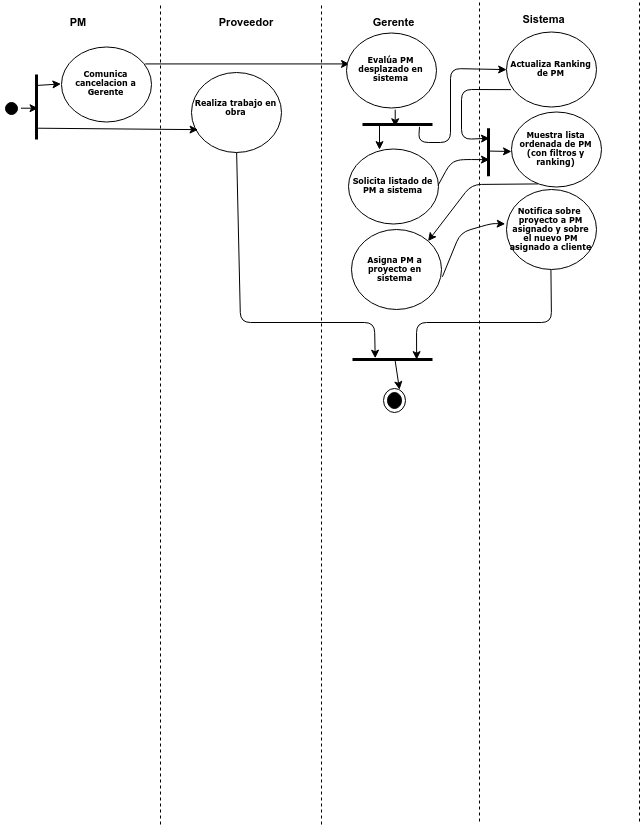
\includegraphics[angle=90]{imagenes/DA4.png}
\end{adjustbox}
\end{center}


\newpage
\section{Maquinas de Estado Finito}
\subsection{Descripción general}

\subsection{Relación con otros modelos}

\subsection{Observaciones de las Vistas}


\newpage
\subsection{Vistas}
\begin{center}
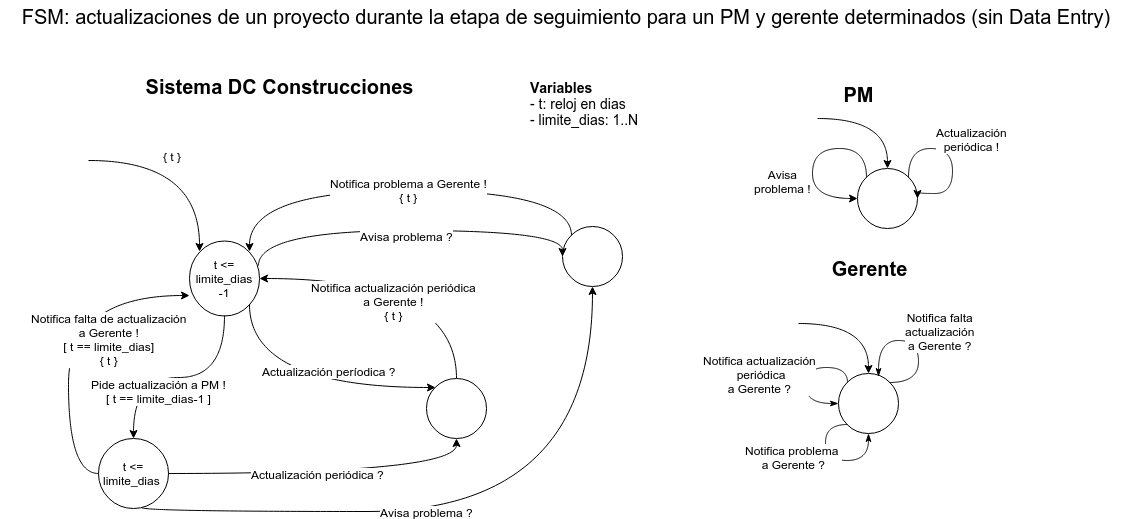
\includegraphics[scale=0.5, angle=90]{imagenes/FSM1.png}
\end{center}

\newpage
\begin{center}
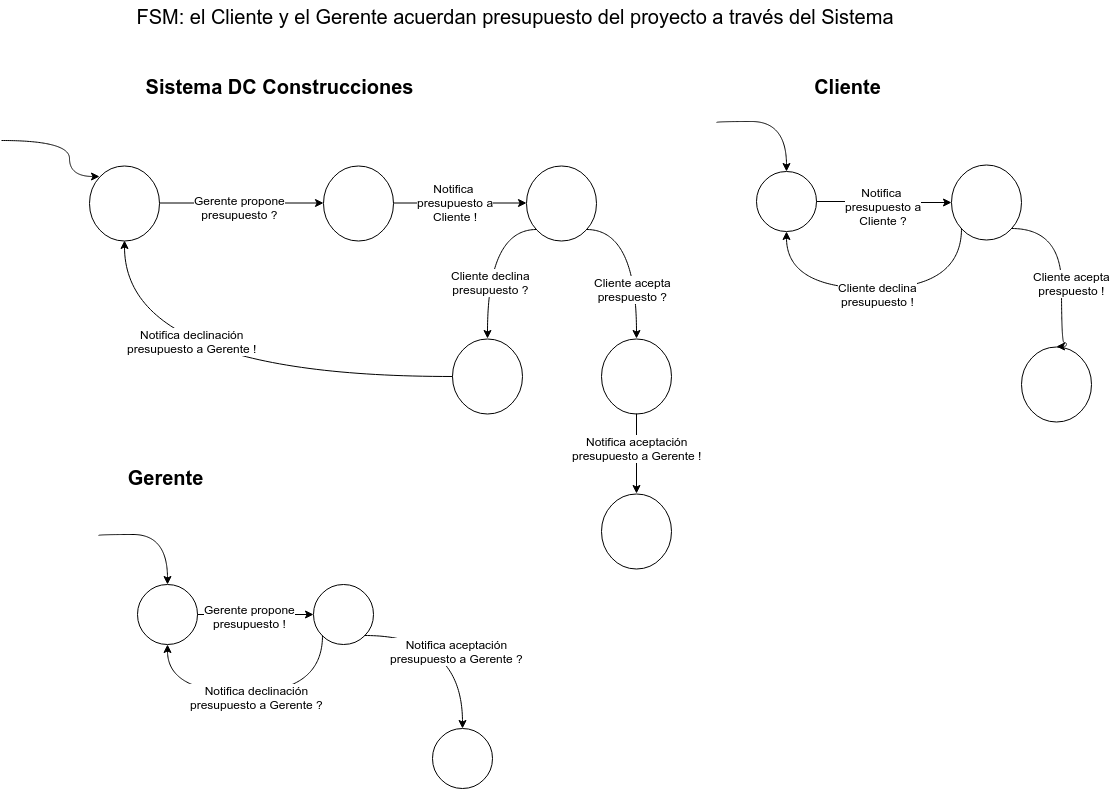
\includegraphics[scale=0.5, angle=90]{imagenes/FSM2.png}
\end{center}

\newpage
\begin{center}
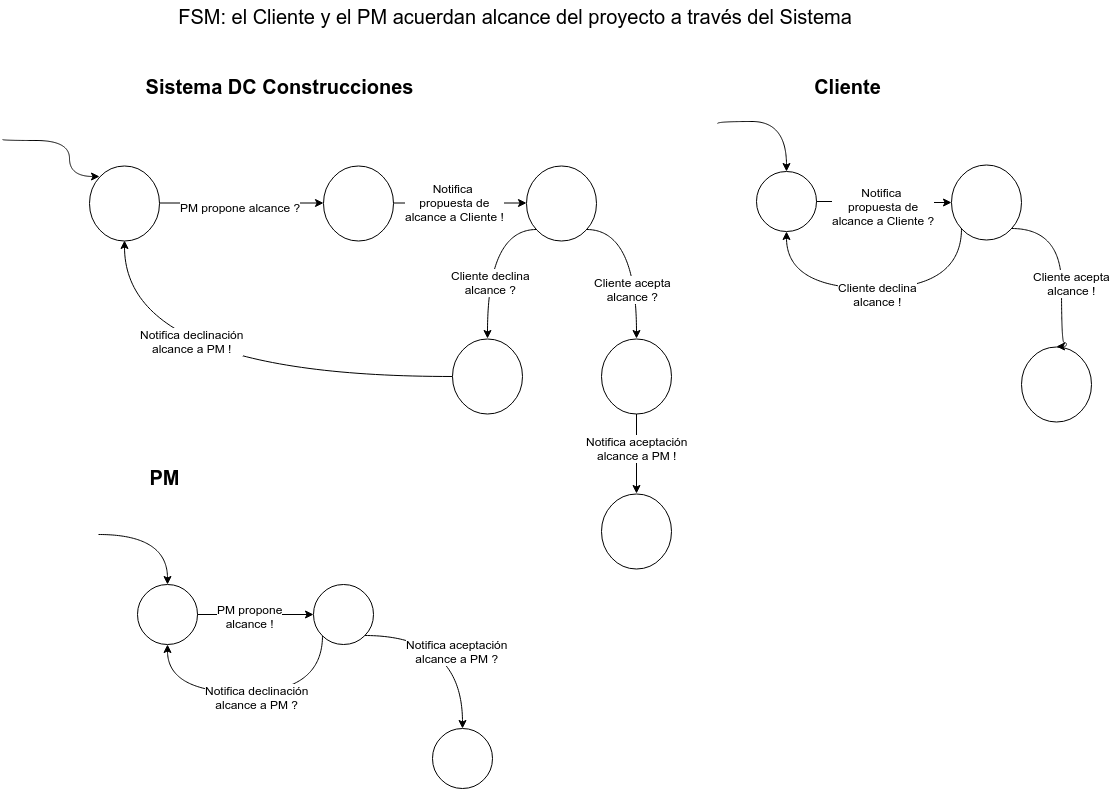
\includegraphics[scale=0.5, angle=90]{imagenes/FSM3.png}
\end{center}


\newpage
\section{Modelo Conceptual}
\subsection{Descripción general}

Este modelo especifica de forma estática los diferentes estados válidos de un proyecto según el sistema. Con eso en mente, nuestro modelo realizado contempla:

\begin{itemize}
	\item Todo los agentes relacionados con el proyecto desde el punto de vista del Sistema
	\item Los presupuestos clientes y proveedores y como se relacionan con los contratos que luego se firman
	\item Comisiones de los PMs
	\item Los rankings de PMs y Proveedores
	\item Seguros de caución de los Proveedores y su validez
	\item Representa estados que muestran cuando hay cambios de PMs y Proovedores
	\item Actualizaciones de Proyecto
	\item Notificaciones periódicas y por problemas
	\item Evaluaciones de proyecto cuando el mismo finaliza
	\item Los estados y propiedades de un proyecto y todos sus agentes relacionados según el Sistema
\end{itemize}

Nuestro modelo conceptual tiene como principal clase el Proyecto, que es el eje de todo el Sistema y el agente con mas relaciones con los demás. A su vez, se modelan los presupuestos y contratos con los proveedores y clientes. Determinamos que cada presupuesto de un Proveedor es para un proyecto diferente pero que un Cliente puede tener varios presupuestos propuestos para un mismo proyecto. En caso de que esos presupuestos sean aprobados, se crea un Contrato para ese presupuesto (cosa que marcamos con una relación 0..1 contratoCliente/contratoProveedor).

Cada proyecto en sí tiene un Gerente que lo supervisa y un PM actual (pueden haber varios PMs relacionados mediante la clase Comision, pero solo uno es el actual, los demás están porque fueron PMs y en algun momento fueron cancelados). Este PM puede subir actualizaciones de Proyecto y por cada una se genera una actualización.

También modelamos los rankings de Proveedores y PMs, evaluaciones al terminar el proyecto y notificaciones según el agente que la recibe (es decir, si hay una notificación para, por ejemplo, un Gerente y un PM, se generan dos notificaciones distintas en este modelo, una para el Gerente y otra para el PM).
El caso de los Contadores decidimos modelarlo relacionándolo al Gerente y no al Proyecto porque el Contador ayuda el Gerente y las cobranzas y pagos lo realiza todo externamente al Sistema.

El caso en que un nuevo PM es asignado para un proyecto, se marca la Comisión del viejo PM como cancelada (mediante una propiedad de estado) y se agrega una Comisión a otro PM. En cambio, cuando hay un cambio de Proveedor, el Contrato de ese Proveedor es el que se marca como cancelado (también mediante una propiedad de estado).

Consideramos que tanto los contratos de los Proveedores pueden ser cancelados como los de los Clientes. En el primer caso porque un Proveedor puede ser removido de la obra y cambiado por otros. En el segundo porque al renegociar con nuevos Proveedores (cuando estos cambian), también hay que firmar un nuevo contrato con el cliente.

Notar que los Data Entries no los modelamos pues no eran relevantes para el Proyecto en sí.

\subsection{Relación con otros modelos}
Ahora bien, como explicabamos antes, el modelo conceptual modela los estados, propiedades y relaciones estáticas entre los agentes de un proyecto según el Sistema. Por esto mismo, hay cosas que los demás modelos especifican de forma mas precisa:

Las etapas previas a la creación de un proyecto, el acuerdo de alcance y duración del proyecto con el PM se ven mucho mejor en los diagramas de FSM y Actividad, de hecho, el alcance lo modelamos asumiendo que guardar todos los alcances acordados y re-acordados del Proyecto para el Modelo Conceptual es irrelevante y solo nos interesa el alcance actual, es decir el último acordado.
La autenticación y los procedimientos de un Usuario en el Sistema y cómo se usa el Sistema en si, está explicado más claramente en el Diagrama de Casos de Uso.

Las notificaciones, como esto afecta al sistema y qué eventos las causan se pueden ver explícitamente en los Diagramas de FSM. 

Los Data Entries también son modelados en los demás Diagramas. 

La cronología en general de todos los eventos del proyecto se explica mejor en el Diagrama de Actividad.

%Los pagos y cobranzas del Contador a cada parte (Cliente, PM, Gerente, Proveedores) se especifica en el Diagrama de Actividad.

\subsection{Observaciones de las Vistas}
Como se puede ver, hay tres vistas para el Diagrama de Clases, pero estas tres vistas forman en realidad parte de un solo diagrama. Las separamos por motivos de claridad pero tienen que ser leídas e interpretadas como parte de un mismo Diagrama de Clases. Por este motivo, marcamos con números las clases que se repiten en las vistas para decir que en realidad son las mismas clases y que todo es parte de un solo y mismo diagrama.

\newpage
\subsection{Vistas}
\begin{center}
\includegraphics[scale=0.5, angle=90]{imagenes/ModeloConceptual1.png}
\end{center}
\newpage
\begin{center}
\includegraphics[scale=0.5, angle=90]{imagenes/ModeloConceptual2.png}
\end{center}
\newpage
\begin{center}
\includegraphics[scale=0.5, angle=90]{imagenes/ModeloConceptual3.png}
\end{center}

\newpage
\subsection{OCL}
Nuestro modelo tendrá las siguientes restricciones:

\begin{listocl}

\begin{itemocl}{Los rankings de Proveedor están bien formados (tienen del número 1 a cantidad(Proveedores)).}
Context: Proveedor
Inv: Proveedor.allInstances()->isUnique(posicionProv.numero) and Proveedor.allInstances()->exists(p | p.posicionProv.numero = 1) and Proveedor.allInstances()->exists(p | p.posicionProv.numero = Proveedor.allInstances()->size())
\end{itemocl}

\begin{itemocl}{Los rankings de PMs están bien formados (tienen del número 1 a cantidad(PMs)).}
Context: PM
Inv: PM.allInstances()->isUnique(posicionPM.numero) and PM.allInstances()->exists(p | p.posicionPM.numero = 1) and PM.allInstances()->exists(p | p.posicionPM.numero = PM.allInstances()->size())
\end{itemocl}

\begin{itemocl}{Cada proveedor tiene un seguro de caución que vence después de la finalización de cada proyecto al que le mandó un presupuesto.}
Context: Proveedor
Inv: self.presupuestos->collect(presupuestoProvDe)->forAll(proy | self.seguros->exists(seg | seg.fechaVencimiento >= proy.fechaFin))
\end{itemocl}

\begin{itemocl}{Los contratos de Proveedores están asociados a un gerente que supervisa el proyecto del contrato.}
Context: ContratoProveedor
Inv: self.gerenteInvolucrado.supervisa->includes(self.presupuesto.presupuestoProvDe)
\end{itemocl}

\begin{itemocl}{Los contratos de Clientes están asociados a un gerente que supervisa el proyecto del contrato.}
Context: ContratoCliente
Inv: self.gerenteInvolucrado.supervisa->includes(self.presupuesto.presupuestoClienteDe)
\end{itemocl}

\begin{itemocl}{Cada proveedor manda como máximo un presupuesto por proyecto.}
Context: Proveedor
Inv: self.presupuestos->isUnique(presupuestoProvDe)
\end{itemocl}

\begin{itemocl}{Hay como máximo un presupuesto del cliente con contrato firmado (y no cancelado) para cada proyecto.}
Context: Proyecto
Inv: self.presupuestosCliente->select(pres | pres.contrato->notEmpty() and pres.contrato.estado = firmado)->size() <= 1
\end{itemocl}

\begin{itemocl}{Si el proyecto no empezo, no hay contrato de clientes firmados, si empezo hay exactamente un contrato de cliente firmado y al menos un contrato de Proveedor firmado.}
Context: Proyecto
Inv: self.estado = noEmpezo implies self.presupuestosCliente->select(pres | pres.contrato->notEmpty() and pres.contrato.estado = firmado)->size() = 0 and self.estado <> noEmpezo implies (self.presupuestosCliente->select(pres | pres.contrato->notEmpty() and pres.contrato.estado = firmado)->size() = 1 and self.presupuestosProv->select(pres | pres.contrato->notEmpty() and pres.contrato.estado = firmado)->size() > 0)
\end{itemocl}

\begin{itemocl}{La suma de los presupuestos de los Proveedores que firmaron un contrato es menor al presupuesto que se le manda al cliente.}
Context: Proyecto
Inv: self.presupuestosCliente->select(presCliente | presCliente.contrato->notEmpty() and presCliente.contrato.estado = firmado)->forall(presCliente | presCliente.monto < self.presupuestosProv->select(presProv | presProv.contrato->notEmpty() and presProv.contrato.estado = firmado)->collect(monto)->sum())
\end{itemocl}

\begin{itemocl}{El cliente de un proyecto coincide con el cliente asociado a cada presupuesto del proyecto.}
Context: Proyecto
Inv: self.presupuestosCliente->forAll(pres | pres.cliente = self.cliente)
\end{itemocl}

\begin{itemocl}{Hay como máximo un PM actual por proyecto (puede ser momentaneamente ninguno cuando se cambia de PM).}
Context: Proyecto
Inv: self.comisionesProyecto->select(c | c.estado = actual) <= 1
\end{itemocl}

\begin{itemocl}{Cada comisión de un PM es para un proyecto distinto.}
Context: PM
Inv: self.comisionesPM->isUnique(proyecto)
\end{itemocl}

\begin{itemocl}{Todas las actualizaciones de Proyecto pertenecen a un PM que es o fue el PM asignado del proyecto de la actualización.}
Context: PM
Inv: self.actualizaciones->forAll(a | self.comisionesPM->exists(c | c.proyecto = a.actualizacionDe))
\end{itemocl}

% ----------- Evaluaciones

\begin{itemocl}{Las evaluaciones de Gerentes a PMs están en un ciclo válido (es decir, el PM y el Gerente estuvieron asignados al proyecto de la evaluación).}
Context: EvaluacionGerentePM
Inv: self.PM.comisionesPM->collect(proyecto)->includes(self.proyecto) and self.gerente.supervisa->includes(self.proyecto)
\end{itemocl}

\begin{itemocl}{Las evaluaciones de Clientes a PMs están en un ciclo válido (es decir, el Cliente y el Gerente estuvieron asignados al proyecto de la evaluación).}
Context: EvaluacionClientePM
Inv: self.PM.comisionesPM->collect(proyecto)->includes(self.proyecto) and self.cliente = self.proyecto.cliente
\end{itemocl}

\begin{itemocl}{Las evaluaciones de Gerentes a PMs están en un ciclo válido (es decir, el PM y el Gerente estuvieron asignados al proyecto de la evaluación).}
Context: EvaluacionPMProveedor
Inv: self.PM.comisionesPM->collect(proyecto)->includes(self.proyecto) and self.proyecto.presupuestosProv->select(p | p.contrato->notEmpty())->includes(self.proveedor)
\end{itemocl}

\begin{itemocl}{Por cada PM cancelado hay una evaluación del Cliente al PM y otra del Gerente al PM.}
Context: Comision
Inv: self.estado = cancelada implies (self.proyecto.evalsGerPMProyecto->exists(e | e.PM = self.comisionDe) and self.proyecto.evalsClientePMProyecto->exists(e | e.PM = self.comisionDe))
\end{itemocl}

\begin{itemocl}{Por cada Proveedor cancelado hay una evaluación del PM a ese Proveedor.}
Context: ContratoProveedor
Inv: self.estado = cancelado implies self.presupuesto.presupuestoProvDe.evalsPMProvProyecto->exists(e | e.proveedor = self.presupuesto.proveedor)
\end{itemocl}

\begin{itemocl}{Si el proyecto terminó, se evaluaron a todos los PMs y Proveedores involucrados.}
Context: Proyecto
Inv: self.estado = terminado implies (self.comisionesProyecto->collect(comisionDe)->forAll(pm | self.evalsGerPMProyecto->includes(e | e.PM = pm) and self.evalsClientePMProyecto->exists(e | e.PM = pm)) and self.presupuestosProv->select(pres | pres.contrato->notEmpty())->collect(proveedor)->forAll(prov | self.evalsPMProvProyecto->exists(e | e.proveedor = prov)))
\end{itemocl}

% ----------- Notificaciones

\begin{itemocl}{Fechas correctas: la fecha de inicio de un proyecto es menor que la de finalización, las fechas de las actualizaciones y notificaciones son mayores o iguales a la fecha de inicio del proyecto}
Context: Proyecto
Inv: self.fechaFin < self.fechaInicio and self.actualizaciones->forAll(a | a.fecha >= self.fechaInicio) and self.notisGerenteProyecto->forAll(n | n.fecha >= self.fechaInicio) and self.notisClienteProyecto->forAll(n | n.fecha >= self.fechaInicio) and self.notisPMProyecto->forAll(n | n.fecha >= self.fechaInicio) and self.notisProvProyecto->forAll(n | n.fecha >= self.fechaInicio)
\end{itemocl}

% Nueva propuesta al Gerente
% Asignación de PM al PM y al Cliente
% Propuesta de alcance al Cliente
% Aceptacion de alcance de Cliente al PM
% Aceptacion de presupuesto de Cliente al Gerente
% Finalizacion de Proyecto a Gerente
% Existencia de problema al Gerente
% A proveedor cuando seguro vencido
% Respuesta del Proveedor al PM
% Proveedores elegidos a Proveedores
% Proyecto validado a Cliente, PMs y Proveedores

\begin{itemocl}{Las notificaciones a Gerentes son al asignado del proyecto.}
Context: NotificacionGerente
Inv: self.gerente = self.proyecto.gerente
\end{itemocl}

\begin{itemocl}{Las notificaciones a Clientes son al del proyecto.}
Context: NotificacionCliente
Inv: self.cliente = self.proyecto.cliente
\end{itemocl}

\begin{itemocl}{Las notificaciones a PMs son a alguno asignado en algún momento al proyecto.}
Context: NotificacionPM
Inv: self.proyecto.comisionesProyecto->collect(comisionDe)->exists(pm | pm = self.PM)
\end{itemocl}

\begin{itemocl}{Las notificaciones a Proveedores son a alguno asignado alguna vez al proyecto.}
Context: NotificacionProveedor
Inv: self.proyecto.presupuestosProv->select(p | p.contrato->notEmpty())->collect(proveedor)->exists(prov | prov = self.proveedor)
\end{itemocl}

\end{listocl}

Aclaraciones: según nuestro modelo, no es necesario restringir con OCL que ciertos eventos causan un envío de nootificaciones porque es un comportamiento deseado pero no un comportamiento necesario para que la instancia del sistema sea válida. Mediante los otros Diagramas (como el de Actividad) especificamos que ciertos eventos como la creación de un proyecto causa un envío de notificación al Gerente, esto es algo deseado pero no necesario de restringir con OCL.


\newpage
\section{Conclusiones}
El presente Trabajo Práctico se propuso, a partir de los objetivos y requerimientos realizados en el trabajo anterior,
realizar una serie de modelos que permitan:

\begin{itemize}
	\item Entender en detalle cuales son las interacciones que tendrá el Sistema con el resto de los actores.
	\item Entender cuales son los conceptos que se tienen en cuenta dentro del Sistema, y cuales son las relaciones entre ellos.
	\item Entender cual es el ciclo de vida de un proyecto cuando los diferentes actores utilizan el Sistema.
\end{itemize}

Los cuales creemos que se pudieron realizar de manera adecuada. Encontramos que cada modelo tiene ventajas para ciertos escenarios:
\begin{itemize}
	\item El Diagrama de Casos de Uso (junto con el detalle de cada uno de ellos) es esencial para entender cual es la interfaz del Sistema, y ver cual es el detalle fino de las interacciones definidas en el Diagrama de Contexto.
	\item El Diagrama de Actividad es muy útil para entender las interacciones a lo largo del tiempo de varios actores en un proceso determinado. En el caso de este trabajo, se utilizó para mostrar el ciclo de vida completo de un proyecto, y como influye cada actor en las diferentes etapas de este.
	\item El Diagrama de Maquinas de Estado permite dar el detalle de procesos que son muy dinámicos y no son sencillos de expresar con el Diagrama de Actividad. En el caso de este trabajo, se utilizó para mostrar los procesos de: actualizaciones del PM en el seguimiento de un proyecto, y la negociación a través del Sistema del presupuesto (entre Gerente y Cliente) y el alcance del proyecto (entre PM y Cliente).
	\item El Modelo Conceptual muestra cuales son los conceptos a tener en cuenta en un problema, y como se relacionan entre ellos. En el caso de este trabajo, se utilizó para mostrar las relaciones que tienen los distintos actores alrededor del concepto ``Proyecto'', ya que es un concepto central del problema y merece ese nivel de detalle.
\end{itemize}

En cuanto a la trazabilidad entre los distintos diagramas planteados, vimos que muchas veces es difícil mantener la coherencia entre estos, pero que es fundamental para lograr una comprensión entera del problema. Incluso en el caso en el que algunos diagramas definían escenarios similares y se superponían, utilizar diferentes diagramas nos permitió ver estos escenarios desde distintos niveles de perspectiva.

La experiencia que se lleva el grupo de las distintas herramientas utilizadas es que cada una debe ser usada en el contexto adecuado, ya que la realización de los diagramas lleva un tiempo considerable que no parecería justificarse si el escenario no es lo suficientemente complicado, o si el diagrama no aporta mucho más que leer el problema en lenguaje natural.


% \newpage
% \bibliographystyle{plain}
% \section{Referencias}
% \begingroup
% \renewcommand{\section}[2]{}
% \bibliography{informe}
% \endgroup
%
% \newpage
% \appendix
% \input{apendice}

\end{document}
